\documentclass[10pt]{article}
\usepackage[a4paper,margin=12mm]{geometry}
\usepackage{xeCJK}
\setCJKmainfont{Microsoft JhengHei}
\usepackage{amsmath,amssymb}
\usepackage{graphicx}
\usepackage{booktabs}
\usepackage{multirow}
\usepackage[table]{xcolor}
\usepackage{caption}
\usepackage{enumitem}
\graphicspath{{../../paper/fig/}}
\definecolor{oursrow}{HTML}{FCEBEC}
\newcommand{\pend}[1]{#1}
\setlist{nosep,leftmargin=1.5em}
\setlength{\parindent}{0pt}
\captionsetup{labelformat=empty}

\begin{document}

\section*{1. 主比較（Table 1）}
\textbf{設定}
\begin{itemize}
  \item Pexels 306 張（未齊者以現有值，張數標於格右上角）
  \item InstructPix2Pix；四句配件指令
  \item 七道淨化、VAE-Trans
  \item 加性方法：等失真設定
\end{itemize}
\textbf{組別}
\begin{itemize}
  \item DAYN、DIA-R、DIA-PT、SIFM、DANP、Mist、PhotoGuard（encoder）、DCT-Shield、DCT-Shield-Y、Ours
\end{itemize}

\begin{table}[h]
  \centering
  \footnotesize
  \setlength{\tabcolsep}{1.5pt}
  \begin{tabular}{l c cccc cccc c cc c}
    \toprule
    & \textbf{Distortion} & \multicolumn{4}{c}{\textbf{Aesthetics} (no reference)} & \multicolumn{4}{c}{\textbf{Edit LPIPS} $\uparrow$} & & \multicolumn{2}{c}{\textbf{Edit SigLIP} $\downarrow$} & \textbf{Identity} \\
    \cmidrule(lr){2-2} \cmidrule(lr){3-6} \cmidrule(lr){7-10} \cmidrule(lr){12-13} \cmidrule(l){14-14}
    Method & LPIPS $\downarrow$ & LAION $\uparrow$ & NIMA $\uparrow$ & MUSIQ $\uparrow$ & NIQE $\downarrow$ & None & 7-mean & Weakest$^{*}$ & VAE-Trans & Ret.$^{\dagger}$ $\uparrow$ & 7-mean & VAE-Trans & ArcFace $\downarrow$ \\
    \midrule
    \textcolor{gray}{Original} & \textcolor{gray}{--} & \pend{5.478}$^{b}$ & \pend{5.422}$^{b}$ & \pend{5.310}$^{b}$ & \pend{4.576}$^{b}$ & & & & & & & & \\
    \midrule
    DAYN & \pend{.328}$^{b}$ & \pend{5.527}$^{b}$ & \pend{5.205}$^{b}$ & \pend{5.007}$^{b}$ & \pend{4.742}$^{b}$ & \pend{.386}$^{b}$ & \pend{.241}$^{b}$ & \pend{.148}$^{b}$ & \pend{.067}$^{b}$ & \pend{.639}$^{b}$ & \pend{.931}$^{b}$ & \pend{.983}$^{b}$ & \pend{.885}$^{b}$ \\
    DIA-R & \pend{.348}$^{b}$ & \pend{\textbf{5.623}}$^{b}$ & \pend{5.316}$^{b}$ & \pend{5.136}$^{b}$ & \pend{4.752}$^{b}$ & \pend{.390}$^{b}$ & \pend{.229}$^{b}$ & \pend{.105}$^{b}$ & \pend{.055}$^{b}$ & \pend{.603}$^{b}$ & \pend{.943}$^{b}$ & \pend{.989}$^{b}$ & \pend{.895}$^{b}$ \\
    DIA-PT & \pend{.327}$^{b}$ & \pend{5.428}$^{b}$ & \pend{5.295}$^{b}$ & \pend{5.149}$^{b}$ & \pend{\textbf{4.358}}$^{b}$ & \pend{.386}$^{b}$ & \pend{.216}$^{b}$ & \pend{.099}$^{b}$ & \pend{.048}$^{b}$ & \pend{.579}$^{b}$ & \pend{.946}$^{b}$ & \pend{.991}$^{b}$ & \pend{.905}$^{b}$ \\
    SIFM & \pend{.300}$^{b}$ & \pend{5.561}$^{b}$ & \pend{5.335}$^{b}$ & \pend{5.178}$^{b}$ & \pend{4.432}$^{b}$ & \pend{.380}$^{b}$ & \pend{.201}$^{b}$ & \pend{.091}$^{b}$ & \pend{.049}$^{b}$ & \pend{.546}$^{b}$ & \pend{.953}$^{b}$ & \pend{.989}$^{b}$ & \pend{.910}$^{b}$ \\
    DANP & \pend{.308}$^{b}$ & \pend{5.516}$^{b}$ & \pend{5.324}$^{b}$ & \pend{5.130}$^{b}$ & \pend{4.432}$^{b}$ & \pend{.370}$^{b}$ & \pend{.200}$^{b}$ & \pend{.086}$^{b}$ & \pend{.050}$^{b}$ & \pend{.554}$^{b}$ & \pend{.957}$^{b}$ & \pend{.990}$^{b}$ & \pend{.905}$^{b}$ \\
    Mist & \pend{.367}$^{b}$ & \pend{5.556}$^{b}$ & \pend{5.381}$^{b}$ & \pend{\textbf{5.248}}$^{b}$ & \pend{4.576}$^{b}$ & \pend{.400}$^{b}$ & \pend{.185}$^{b}$ & \pend{.057}$^{b}$ & \pend{.037}$^{b}$ & \pend{.465}$^{b}$ & \pend{.958}$^{b}$ & \pend{.993}$^{b}$ & \pend{.929}$^{b}$ \\
    PhotoGuard & \pend{.367}$^{b}$ & \pend{5.566}$^{b}$ & \pend{5.367}$^{b}$ & \pend{5.227}$^{b}$ & \pend{4.623}$^{b}$ & \pend{\textbf{.438}}$^{b}$ & \pend{.179}$^{b}$ & \pend{.059}$^{b}$ & \pend{.040}$^{b}$ & \pend{.420}$^{b}$ & -- & \pend{.993}$^{b}$ & \pend{.931}$^{b}$ \\
    DCT-Shield & \pend{.326}$^{b}$ & \pend{5.564}$^{b}$ & \pend{\textbf{5.414}}$^{b}$ & \pend{5.235}$^{b}$ & \pend{5.347}$^{b}$ & \pend{.322}$^{b}$ & \pend{.129}$^{b}$ & \pend{.037}$^{b}$ & \pend{.030}$^{b}$ & \pend{.408}$^{b}$ & \pend{.970}$^{b}$ & \pend{.995}$^{b}$ & \pend{.937}$^{b}$ \\
    DCT-Shield-Y & \pend{.315}$^{b}$ & \pend{5.418}$^{b}$ & \pend{5.372}$^{b}$ & \pend{5.123}$^{b}$ & \pend{5.085}$^{b}$ & \pend{.291}$^{b}$ & \pend{.128}$^{b}$ & \pend{.041}$^{b}$ & \pend{.034}$^{b}$ & \pend{.451}$^{b}$ & \pend{.969}$^{b}$ & \pend{.992}$^{b}$ & \pend{.937}$^{b}$ \\
    \midrule
    \rowcolor{oursrow}
    \textbf{Ours} & \pend{\textbf{.211}}$^{a}$ & \pend{5.482}$^{b}$ & \pend{5.293}$^{b}$ & \pend{5.241}$^{b}$ & \pend{4.447}$^{b}$ & \pend{.277}$^{a}$ & \pend{\textbf{.291}}$^{a}$ & \pend{\textbf{.251}}$^{a}$ & \pend{\textbf{.301}}$^{b}$ & \pend{\textbf{1.091}}$^{a}$ & \pend{\textbf{.883}}$^{b}$ & \pend{\textbf{.905}}$^{b}$ & \pend{\textbf{.842}}$^{b}$ \\
    \bottomrule
  \end{tabular}

  \smallskip
  未到目標張數的格以現有值填入。$^{a}$Pexels，$n=306$。$^{b}$8 張 portraits，$n=8$。Weakest：加性方法皆為 Gaussian blur $\sigma=2$；Ours 在 $^{a}$ 為 $15^\circ$ 旋轉。
\end{table}

\textbf{說明}：306 張 Pexels 人像 $\times$ 4 句指令（InstructPix2Pix）的主比較；加性方法採其等失真臂的設定。粗體為最佳。$^{*}$平均值最低的一道淨化。$^{\dagger}$保留率。

\clearpage
\section*{2. 失真與編輯位移（Fig. 3）}
\textbf{設定}
\begin{itemize}
  \item 8 張 portraits
  \item InstructPix2Pix；四句配件指令
  \item (a) 淨化前；(b) 淨化前、七道平均
\end{itemize}
\textbf{組別}
\begin{itemize}
  \item (a) 加性方法的原生預算、等失真、預算掃描；Ours
  \item (b) 加性方法的等失真；Ours
\end{itemize}

\begin{center}
  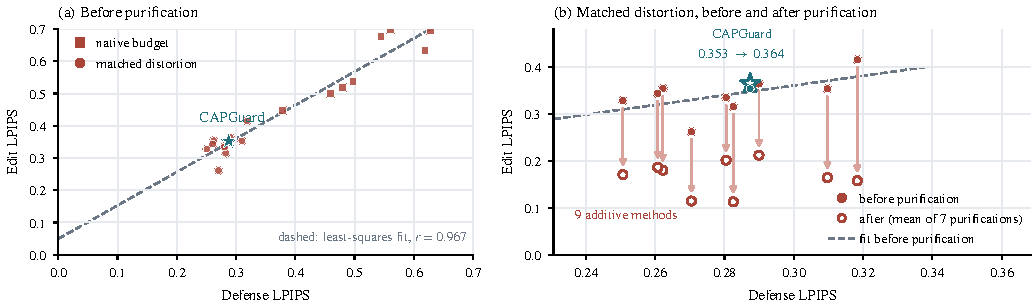
\includegraphics[width=\linewidth]{distortion_displacement.pdf}
\end{center}

\textbf{說明}：InstructPix2Pix 上的失真與編輯位移（8 張 $\times$ 4 句）。(a) 淨化前，加性方法的所有預算點；虛線為最小平方擬合。(b) 等失真臂與 Ours 在淨化前（實心）與淨化後（空心，七道淨化平均）的位置。

\section*{3. 淨化分析（Fig. 4）}
\textbf{設定}
\begin{itemize}
  \item 8 張 portraits
  \item InstructPix2Pix；四句配件指令
  \item (a) 七道淨化、VAE-Trans 的擾動存續比
  \item (b–d) JPEG 95–10、Gaussian blur $\sigma$ 0.5–3、縮放 0.75–0.25
\end{itemize}
\textbf{組別}
\begin{itemize}
  \item (a) DAYN、DIA-R、DIA-PT、SIFM、DANP、Mist、PhotoGuard（encoder）、DCT-Shield、DCT-Shield-Y、Ours
  \item (b–d) DIA-PT、Mist、PhotoGuard（encoder）、DCT-Shield、Ours
\end{itemize}

\begin{center}
  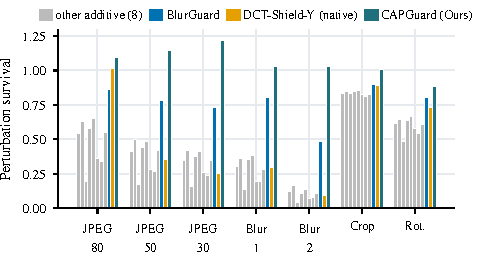
\includegraphics[width=\linewidth]{purification.pdf}
\end{center}

\textbf{說明}：InstructPix2Pix 上淨化的作用（8 張）。(a) 各道淨化後擾動存續的比例。(b–d) JPEG 壓縮、模糊、縮小強度遞增時的編輯 LPIPS（8 張 $\times$ 4 句）；點線為同一張未防禦影像兩個種子之間的編輯 LPIPS。

\clearpage
\section*{4. 不同編碼器的編輯器（Table 2）}
\textbf{設定}
\begin{itemize}
  \item 8 張 portraits
  \item UltraEdit（SD3）、FLUX.1 Kontext；四句配件指令
  \item 七道淨化、VAE-Trans；原生預算
\end{itemize}
\textbf{組別}
\begin{itemize}
  \item PhotoGuard（encoder）、DCT-Shield、DCT-Shield-Y、Mist（textural）、Ours（transfer）、Ours
\end{itemize}

\begin{table}[h]
  \centering
  \footnotesize
  \setlength{\tabcolsep}{4pt}
  \begin{tabular}{l ccccc ccccc}
    \toprule
    & \multicolumn{5}{c}{\textbf{UltraEdit} (Stable Diffusion 3)} & \multicolumn{5}{c}{\textbf{FLUX.1 Kontext}} \\
    \cmidrule(lr){2-6} \cmidrule(l){7-11}
    & Distortion & \multicolumn{3}{c}{Edit LPIPS $\uparrow$} & & Distortion & \multicolumn{3}{c}{Edit LPIPS $\uparrow$} & \\
    \cmidrule(lr){3-5} \cmidrule(lr){8-10}
    Method & LPIPS $\downarrow$ & None & 7-mean & VAE-Trans & Ret.\ $\uparrow$ & LPIPS $\downarrow$ & None & 7-mean & VAE-Trans & Ret.\ $\uparrow$ \\
    \midrule
    PhotoGuard & \pend{.478} & \pend{.530} & \pend{.322} & \pend{.066} & \pend{.609} & \pend{.407} & \pend{.410} & \pend{.274} & \pend{.105} & \pend{.684} \\
    DCT-Shield & \pend{.480} & \pend{.528} & \pend{.252} & \pend{.061} & \pend{.478} & \pend{.444} & \pend{.423} & \pend{.258} & \pend{.121} & \pend{.620} \\
    DCT-Shield-Y & \pend{.578} & \pend{.603} & \pend{.336} & \pend{.091} & \pend{.558} & \pend{.610} & \pend{\textbf{.491}} & \pend{.339} & \pend{.158} & \pend{.712} \\
    Mist (textural) & \pend{.596} & \pend{\textbf{.609}} & \pend{\textbf{.437}} & \pend{\textbf{.304}} & \pend{.718} & \pend{.519} & \pend{.472} & \pend{.411} & \pend{.322} & \pend{.879} \\
    \midrule
    Ours (transfer) & \pend{\textbf{.296}} & \pend{.348} & \pend{.371} & \pend{.263} & \pend{\textbf{1.086}} & \pend{.296} & \pend{.418} & \pend{\textbf{.418}} & \pend{\textbf{.327}} & \pend{\textbf{1.026}} \\
    \rowcolor{oursrow}
    \textbf{Ours} & \pend{.301} & \pend{.358} & \pend{.370} & \pend{.264} & \pend{1.050} & \pend{\textbf{.269}} & \pend{.394} & \pend{.392} & \pend{.315} & \pend{1.019} \\
    \bottomrule
  \end{tabular}

  \smallskip
  8 張 portraits，$n=8$（32 次編輯；七道 224 次）。
\end{table}

\textbf{說明}：以各編輯器的 VAE 編碼器求解的防禦，原生預算（8 張 $\times$ 4 句）。Ours（transfer）：在 InstructPix2Pix 上求解。Ret.：七道淨化的保留率。

\section*{5. 消融（Table 3）}
\textbf{設定}
\begin{itemize}
  \item 8 張 portraits
  \item InstructPix2Pix；四句配件指令
  \item 七道淨化、VAE-Trans
\end{itemize}
\textbf{組別}
\begin{itemize}
  \item 逐項懲罰、單一常數上界、可行集合投影、色相夾角錐投影、旋轉（Ours）
  \item 單角 $6^\circ$、$9^\circ$／$0^\circ$、$9^\circ$／$3^\circ$、$10^\circ$／$3^\circ$（Ours）
  \item 同類隨機旋轉
\end{itemize}

\begin{table}[h]
  \centering
  \footnotesize
  \setlength{\tabcolsep}{5pt}
  \begin{tabular}{@{}lcccccccc@{}}
    \toprule
    & \multicolumn{2}{c}{Protected} & \multicolumn{4}{c}{Edit LPIPS $\uparrow$} & & \\
    \cmidrule(lr){2-3} \cmidrule(lr){4-7}
    Variant & LPIPS $\downarrow$ & LAION $\uparrow$ & None & 7-mean & Weakest & VAE-Trans & Retention $\uparrow$ & Feasible $\uparrow$ \\
    \midrule
    \multicolumn{9}{@{}l}{\emph{Enforcement of naturalness}} \\
    Penalties & \pend{.287} & \pend{5.653} & \pend{.341} & \pend{.302} & \pend{.265} & \pend{.185} & \pend{.892} & \pend{76} \\
    Single bound & \pend{.296} & \pend{5.374} & \pend{\textbf{.378}} & \pend{.363} & \pend{.330} & \pend{.276} & \pend{.965} & -- \\
    Adaptive set & \pend{.326} & \pend{\textbf{5.705}} & \pend{.369} & \pend{.327} & \pend{.273} & \pend{.237} & \pend{.890} & \pend{\textbf{109}} \\
    Hue cone & \pend{.291} & \pend{5.423} & \pend{.350} & \pend{.318} & \pend{.282} & \pend{.211} & \pend{.907} & -- \\
    \rowcolor{oursrow}
    Rotation (ours) & \pend{.296} & \pend{5.482} & \pend{.374} & \pend{.367} & \pend{\textbf{.339}} & \pend{.301} & \pend{1.020} & -- \\
    \midrule
    \multicolumn{9}{@{}l}{\emph{Rotation bounds} (polar / azimuth)} \\
    Single, $6^\circ$ & \pend{.307} & \pend{5.377} & \pend{.373} & \pend{\textbf{.389}} & \pend{.323} & \pend{\textbf{.329}} & \pend{\textbf{1.068}} & -- \\
    $9^\circ$ / $0^\circ$ & \pend{\textbf{.270}} & \pend{5.489} & \pend{.350} & \pend{.342} & \pend{.308} & \pend{.281} & \pend{1.022} & -- \\
    $9^\circ$ / $3^\circ$ & \pend{.280} & \pend{5.500} & \pend{.356} & \pend{.353} & \pend{.324} & \pend{.286} & \pend{1.029} & -- \\
    \rowcolor{oursrow}
    $10^\circ$ / $3^\circ$ (ours) & \pend{.296} & \pend{5.482} & \pend{.374} & \pend{.367} & \pend{\textbf{.339}} & \pend{.301} & \pend{1.020} & -- \\
    \midrule
    Random rotation & \pend{.296} & \pend{5.377} & \pend{.366} & \pend{.368} & \pend{.333} & \pend{.285} & \pend{1.028} & -- \\
    \bottomrule
  \end{tabular}

  \smallskip
  8 張 portraits，$n=8$。Feasible：只適用於有約束的形式；「--」表示該形式沒有約束，或求解紀錄未記錄。
\end{table}

\textbf{說明}：消融（8 張 $\times$ 4 句，InstructPix2Pix）。Feasible：最佳化過程 180 次檢查中所有約束同時成立的次數（各影像平均）。

\clearpage
\section*{6. 補充材料：CLIP-IQA}
\textbf{設定}
\begin{itemize}
  \item 8 張 portraits
  \item InstructPix2Pix；四句配件指令
  \item pyiqa clipiqa：防禦圖；編輯的淨化前、七道平均、VAE-Trans
\end{itemize}
\textbf{組別}
\begin{itemize}
  \item 原圖／未防禦編輯、DAYN、DIA-R、DIA-PT、SIFM、DANP、Mist、PhotoGuard（encoder）、DCT-Shield、DCT-Shield-Y、Ours
\end{itemize}

\begin{table}[h]
  \centering
  \footnotesize
  \setlength{\tabcolsep}{5pt}
  \begin{tabular}{lcccc}
    \toprule
    & Protected & \multicolumn{3}{c}{Edit} \\
    \cmidrule(lr){2-2} \cmidrule(l){3-5}
    Method & image $\uparrow$ & None & 7-mean & VAE-Trans \\
    \midrule
    \textcolor{gray}{Original / undefended} & \pend{.748} & \pend{.788} & \pend{.646} & \pend{.763} \\
    \midrule
    DAYN & \pend{.635} & \pend{.700} & \pend{.603} & \pend{.769} \\
    DIA-R & \pend{.732} & \pend{\textbf{.769}} & \pend{\textbf{.643}} & \pend{\textbf{.770}} \\
    DIA-PT & \pend{.721} & \pend{.650} & \pend{.628} & \pend{.768} \\
    SIFM & \pend{.717} & \pend{.747} & \pend{.634} & \pend{.765} \\
    DANP & \pend{.708} & \pend{.742} & \pend{.635} & \pend{.762} \\
    Mist & \pend{\textbf{.739}} & \pend{.695} & \pend{.634} & \pend{.766} \\
    PhotoGuard & \pend{.721} & \pend{.661} & \pend{.619} & \pend{.764} \\
    DCT-Shield & \pend{.688} & \pend{.681} & \pend{.637} & \pend{.764} \\
    DCT-Shield-Y & \pend{.644} & \pend{.685} & \pend{.639} & \pend{.762} \\
    \midrule
    \rowcolor{oursrow}
    Ours & \pend{.668} & \pend{.761} & \pend{.625} & \pend{.759} \\
    \bottomrule
  \end{tabular}

  \smallskip
  8 張 portraits，$n=8$。
\end{table}

\textbf{說明}：等失真下的 CLIP-IQA（8 張；編輯為 8 張 $\times$ 4 句）。第一列為原圖與未防禦編輯。

\section*{7. 補充材料：FID／KID}
\textbf{設定}
\begin{itemize}
  \item 8 張 portraits
  \item piq InceptionV3 pool3；防禦圖對原圖 8 對 8，編輯 32 對 32
  \item 淨化前、七道平均、VAE-Trans
\end{itemize}
\textbf{組別}
\begin{itemize}
  \item DAYN、DIA-R、DIA-PT、SIFM、DANP、Mist、PhotoGuard（encoder）、DCT-Shield、DCT-Shield-Y、Ours
\end{itemize}

\begin{table}[h]
  \centering
  \footnotesize
  \setlength{\tabcolsep}{4pt}
  \begin{tabular}{l cc cc cc cc}
    \toprule
    & \multicolumn{2}{c}{Protected vs.\ original} & \multicolumn{6}{c}{Defended vs.\ undefended edits} \\
    \cmidrule(lr){2-3} \cmidrule(l){4-9}
    & & & \multicolumn{2}{c}{None} & \multicolumn{2}{c}{7-mean} & \multicolumn{2}{c}{VAE-Trans} \\
    \cmidrule(lr){4-5} \cmidrule(lr){6-7} \cmidrule(l){8-9}
    Method & FID $\downarrow$ & KID $\downarrow$ & FID $\uparrow$ & KID $\uparrow$ & FID $\uparrow$ & KID $\uparrow$ & FID $\uparrow$ & KID $\uparrow$ \\
    \midrule
    DAYN & \pend{39.3} & \pend{-.066} & \pend{86.6} & \pend{-.004} & \pend{51.3} & \pend{-.012} & \pend{19.3} & \pend{-.017} \\
    DIA-R & \pend{32.4} & \pend{-.069} & \pend{73.8} & \pend{-.007} & \pend{45.7} & \pend{-.013} & \pend{12.3} & \pend{-.018} \\
    DIA-PT & \pend{26.6} & \pend{-.072} & \pend{81.7} & \pend{-.000} & \pend{45.3} & \pend{-.012} & \pend{11.3} & \pend{-.018} \\
    SIFM & \pend{20.1} & \pend{-.077} & \pend{76.7} & \pend{-.009} & \pend{40.9} & \pend{-.015} & \pend{14.2} & \pend{-.018} \\
    DANP & \pend{22.7} & \pend{-.075} & \pend{67.1} & \pend{-.009} & \pend{38.6} & \pend{-.015} & \pend{12.3} & \pend{-.017} \\
    Mist & \pend{12.5} & \pend{-.082} & \pend{92.4} & \pend{\textbf{.010}} & \pend{36.3} & \pend{-.014} & \pend{10.0} & \pend{-.018} \\
    PhotoGuard & \pend{16.5} & \pend{-.079} & \pend{\textbf{102.6}} & \pend{-.005} & \pend{37.5} & \pend{-.014} & \pend{10.3} & \pend{-.018} \\
    DCT-Shield & \pend{\textbf{6.6}} & \pend{\textbf{-.083}} & \pend{65.0} & \pend{-.010} & \pend{26.9} & \pend{-.016} & \pend{8.2} & \pend{-.018} \\
    DCT-Shield-Y & \pend{7.7} & \pend{-.080} & \pend{54.5} & \pend{-.010} & \pend{26.9} & \pend{-.017} & \pend{9.8} & \pend{-.018} \\
    \midrule
    \rowcolor{oursrow}
    Ours & \pend{75.9} & \pend{-.056} & \pend{75.4} & \pend{-.008} & \pend{\textbf{70.6}} & \pend{\textbf{-.008}} & \pend{\textbf{64.9}} & \pend{\textbf{-.011}} \\
    \bottomrule
  \end{tabular}

  \smallskip
  8 張 portraits，$n=8$。KID 在此張數下為負值或接近 0（逐張配對、$n \le 32$ 的無偏估計），只列出不作比較。七道欄為 7 組的平均。
\end{table}

\textbf{說明}：等失真下的 FID 與 KID（piq，InceptionV3 pool3）。防禦圖對原圖為 8 對 8 張；編輯為 32 對 32 次。防禦後與未防禦編輯之間的距離越大，代表位移越大。

\end{document}
